\documentclass{beamer}
%\documentclass[8pt]{beamer}
\usepackage{graphicx}

%THEME and COLORTHEME
\usetheme{Madrid}
%\usetheme{Berkeley}
%\usetheme{Copenhagen}

% \usecolortheme{beaver}
% \usecolortheme{beetle}
%\usecolortheme{seahorse}
%\usecolortheme{wolverine}

%DEMO TITLEPAGE
%Information to be included in the title page:
% \title{Title}
% \author{Author}
% \institute{Institute}
% \date{\today}

%FIXING TITLEPAGE
\title{Class on LaTeX: Beamer}

\subtitle{An Introduction}

\author[M. Nahar]{Mahjabin Nahar}
%\author{A.~B \and X.~Y}

\institute[Bangladesh]
{
  Department of Computer Science and Engineering\\
  Bangladesh University of Engineering and Technology
}

\date{\today}

\logo{
\includegraphics[height=1cm]{overleaf.png}}

% PLACING ToC AT THE BEGINNING OF EACH SECTION
% \AtBeginSection[]
% {
%   \begin{frame}
%     \frametitle{Table of Contents}
%     \tableofcontents[currentsection]
%   \end{frame}
% }

\begin{document}

\frame{\titlepage}

%FRAME AND FIGURE
% \begin{frame}{Frame 1}
% This is some text in the first frame. 
% \end{frame}

% \begin{frame}{Frame 2}
% \begin{figure}[h]
% 	\centering
% 	\caption{This caption is at the top}
% 	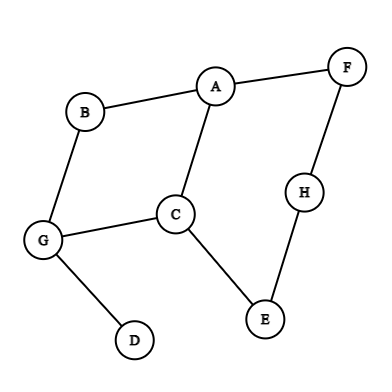
\includegraphics[scale=0.4]{graph.png}
% 	\label{fig:1}
% 	%\caption{This is figure 1.}
% \end{figure}
% \end{frame}

%TABLE OF CONTENTS
\begin{frame}
\frametitle{Table of Contents}
\tableofcontents
\end{frame}

\section{First Section}
\begin{frame}{First Section: Frame 1}
This is some text in the first frame. 
\end{frame}

\section{Second Section}
\subsection{Subsection 1: Hibi}
\begin{frame}{Second Section: Frame 1}
\begin{figure}[h]
	\centering
	\caption{This caption is at the top}
	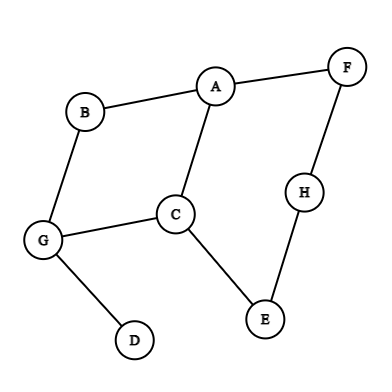
\includegraphics[scale=0.4]{graph.png}
	\label{fig:1}
	%\caption{This is figure 1.}
\end{figure}
\end{frame}
\subsection{Subsection 2: Jibi}
% %EFFECTS DEMO
\begin{frame}{Second Section: Frame 2}
This is a sample line of text.

\begin{itemize}
 \item<1->
 \item<1-> Text visible from slide 1 
 \item<2-> Text visible from slide 2
 \item<3> Text visible on slide 3
 \item<4-5> Text visible on slides 4 and 5
 \item<5-> Text visible from slide 5
 \item<6-> Text visible from slide 6
\end{itemize}
\end{frame}

% %EFFECTS DEMO USING PAUSE
\begin{frame}{Second Section: Frame 3}
 In this slide \pause

 the text will be partially visible \pause

 And finally everything will be there
\end{frame}

% %TWO COLUMN SLIDE
\begin{frame}{Second Section: Frame 4}

\begin{columns}
\column{0.5\textwidth}
This is a text in the first column.
$$E=mc^2$$
This is a list.
\begin{itemize}
\item First item
\item Second item
\end{itemize}

\column{0.5\textwidth}
This text will be in the second column.
This is a nice looking
layout in some cases.
\end{columns}
\end{frame}
\section{Second Section}
\begin{frame}
D
\end{frame}
\section{Second Section}
\begin{frame}
I
\end{frame}
\section{Second Section}
\begin{frame}
N
\end{frame}
\section{Second Section}
\begin{frame}
-THE DAY
\end{frame}
% %BLOCK AND ALERT COMMANDS
\begin{frame}{Second Section: Frame 5}

In this slide, some important text will be
\alert{highlighted} because it's important.

\begin{block}{Remark}
Its a simple facebook group.
\end{block}

\begin{alertblock}{Important theorem}
Sample text in red box
\end{alertblock}

\begin{examples}
Sample text in green box. 
\end{examples}
\end{frame}

\end{document}